\documentclass[11pt,spanish,a4paper]{article}
% Versión 2.o cuat 2015 Víctor Bettachini < bettachini@df.uba.ar >

\usepackage{babel}
\addto\shorthandsspanish{\spanishdeactivate{~<>}}
\usepackage[utf8]{inputenc}
\usepackage{float}

\usepackage{units}
\usepackage[separate-uncertainty=true, multi-part-units=single, locale=FR]{siunitx}

\usepackage{amsmath}
\usepackage{amstext}
\usepackage{amssymb}

\newcommand{\pvec}[1]{\vec{#1}\mkern2mu\vphantom{#1}}

\usepackage{tikz}
% \input{DimLinesTikz}
\usetikzlibrary{decorations.pathmorphing, patterns}

\usepackage{graphicx}
\graphicspath{{./graphs/}}

\usepackage[margin=1.3cm,nohead]{geometry}
% \voffset-3.5cm
% \hoffset-3cm
% \setlength{\textwidth}{17.5cm}
% \setlength{\textheight}{27cm}

\usepackage{lastpage}
\usepackage{fancyhdr}
\pagestyle{fancyplain}
\fancyhead{}
\fancyfoot{{\tiny \textcopyright Departamento de Física, FCEyN, UBA}}
\fancyfoot[C]{ {\tiny Actualizado al \today} }
\fancyfoot[RO, LE]{Pág. \thepage/\pageref{LastPage}}
\renewcommand{\headrulewidth}{0pt}
\renewcommand{\footrulewidth}{0pt}

% \def \materia {Física II para químicos}
\def \periodo {cuatrimestre de verano - 2017}
\def \website {http://materias.df.uba.ar/f2qa2017v}


\begin{document}
\noindent
% \textbf{\materia}\hfill \periodo
\textbf{Física II (Químicos)}\hfill \textcopyright {\tt DF, FCEyN, UBA}
\begin{center}
  \textsc{\large Ley de Coulomb - Campo eléctrico de cargas puntuales - Campo de distribuciones de cargas - Ley de Gauss - Potencial electrostático - Expansión multipolar - Dipolo - Momento dipolar de moléculas}
  % \textsc{\large Guía 1: Ley de Coulomb - Campo eléctrico de cargas puntuales - Campo de distribuciones de cargas - Ley de Gauss - Potencial electrostático - Expansión multipolar - Dipolo - Momento dipolar de moléculas}
\par\end{center}{\large \par}


\begin{enumerate}
% \begin{enumerate}[label=\bfseries Problema \arabic*:]
% \begin{description}

\section*{Ley de Coulomb - Campo eléctrico de cargas puntuales}

  \item \setlength{\parskip}{0cm}
  % \item[Problema 1]\hfill
  \begin{enumerate}
    \item Calcular el cociente q/m entre la carga y la masa de dos partículas idénticas que se repelen electrostáticamente con la misma fuerza con que se atraen gravitatoriamente.
		Comparar el valor hallado con el cociente e/m para el electrón.

		Datos: \(\mathrm{G}= \SI{6.7E-11}{\newton\metre\squared\per\kilogram\squared}\) ; \(\mathrm{k} = \SI{9E9}{\newton\metre\squared\per\coulomb\squared}\) ; \(\ \mathrm{m_ e}= \SI{9.11E-31}{\kilogram}\); \(\mathrm{e} = \SI{1.6E-19}{\coulomb}\).
    \item Calcular la fuerza gravitatoria entre dos esferas de \SI{1}{\centi\metre} de diámetro, de cobre, separadas una distancia de \SI{1}{\metre}.
		Si se retirara a cada esfera un electrón por átomo, ¿cuál sería la fuerza de repulsión electrostática entre ambas?

		Datos: \(\mathrm{\delta_{Cu}}= \SI{9}{\gram\per\centi\metre\cubed}\); \(\mathrm{N_A} = \SI{6.02E23}{}\) ; \(\mathrm{A_{Cu}} = 63.5\).
  \end{enumerate}

	\item \begin{minipage}[t][3cm]{0.65\textwidth}
 		En la figura se muestran tres cargas puntuales idénticas, cada una de masa \(m = \SI{0.100}{\kilogram}\) y carga \(+q\), colgadas de tres cuerdas. 
		Si la longitud de las cuerdas izquierda y derecha es \(L = \SI{30}{\centi\metre}\) y el ángulo \(\theta = \SI{45}{\degree}\), determine el valor de \(q\) sabiendo que el sistema se encuentra en equilibrio.
    \end{minipage}
    \begin{minipage}[c][1em][t]{0.3\textwidth}
		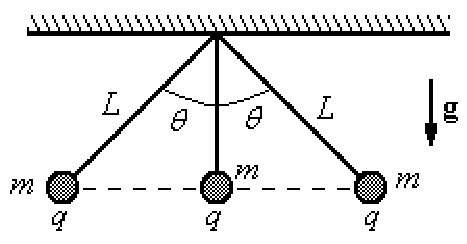
\includegraphics[width=\textwidth]{p1e02}
    \end{minipage}


	\item \begin{minipage}[t][3.5cm]{0.65\textwidth}
		Tres cargas puntuales están ubicadas en los vértices de un triángulo equilátero de \SI{0.5}{\metre} de lado, como indica la figura.
		Calcule la fuerza eléctrica neta sobre la carga de \SI{7}{\micro\coulomb}.
    \end{minipage}
    \begin{minipage}[c][1em][t]{0.3\textwidth}
		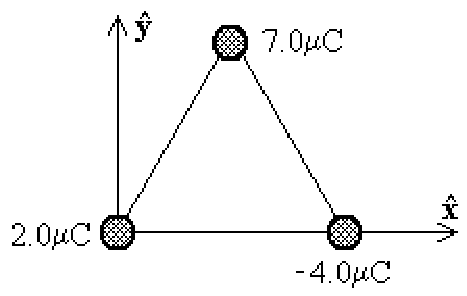
\includegraphics[width=\textwidth]{p1e03}
    \end{minipage}


	\item \begin{minipage}[t][4cm]{0.65\textwidth}
		Cuatro cargas puntuales idénticas (\(q=+\SI{10}{\micro\coulomb}\)) se localizan en las esquinas de un rectángulo, como se indica en la figura.
		Las dimensiones del rectángulo son \(L = \SI{60}{\centi\metre}\) y \(D = \SI{15}{\centi\metre}\).
		Calcule la magnitud y dirección de la fuerza eléctrica neta ejercida sobre la carga en la esquina izquierda inferior por las otras tres cargas. 
    \end{minipage}
    \begin{minipage}[c][1em][t]{0.3\textwidth}
		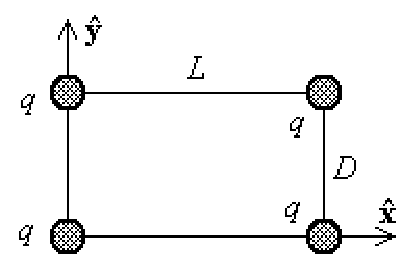
\includegraphics[width=\textwidth]{p1e04}
    \end{minipage}



	\item Halle la fuerza neta sobre una carga \(q\) ubicada en el centro de un cuadrado de lado \(L\), cuando se han colocado cargas \(q, 2q, 4q\) y \(2q\) en los cuatro vértices (en ese orden).
	Saque provecho de la simetría de la configuración de cargas para simplificar el cálculo.


	\item \begin{minipage}[t][4.5cm]{0.7\textwidth}
		Dos cargas puntuales idénticas \(+q\) están fijas en el espacio y separadas por una distancia \(d\).
		Una tercera carga \(–Q\) puede moverse libremente y se encuentra inicialmente en reposo donde muestra la figura, con coordenadas \((x,0)\), a igual distancia de ambas cargas \(+q\).
		Muestre que si \(x\) es pequeña en relación con \(d\), el movimiento de \(–Q\) es armónico simple a lo largo de la recta que equidista de ambas cargas \(+q\) y determine el período de ese movimiento.
    \end{minipage}
    \begin{minipage}[c][1em][t]{0.25\textwidth}
		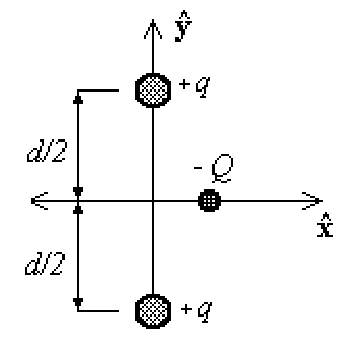
\includegraphics[width=\textwidth]{p1e07}
    \end{minipage}



\item En dos vértices contiguos de un cuadrado de lado \(L\) se hallan dos cargas \(q\).
% \item[Problema 8] En dos vértices contiguos de un cuadrado de lado \(L\) se hallan dos cargas \(q\).
En los dos vértices restantes se colocan dos cargas \(–q\).
Determine, empleando razonamientos de simetría, cuál será la dirección y el sentido del campo eléctrico sobre los ejes perpendiculares a los lados del cuadrado por el punto medio de los mismos.
Calcule el campo eléctrico sobre dichos ejes.


\section*{Campo de distribuciones de cargas}

\item Un hilo muy fino de longitud \(L\) está cargado uniformemente con una carga total \(Q\).
% \item[Problema 9] Un hilo muy fino de longitud L está cargado uniformemente con una carga total \(Q\).
Calcular el campo eléctrico sobre el plano medio del hilo.


\item Una corona circular de radios \(a\) y \(b\) tiene una densidad de carga uniforme \(\sigma\).
% \item[Problema 10] Una corona circular de radios \(a\) y \(b\) tiene una densidad de carga uniforme \(\sigma\).
\begin{enumerate}
  \item Hallar el campo eléctrico en su eje.
  \item Deducir del resultado anterior el campo eléctrico en el eje de un disco de radio \(b\) y luego el campo eléctrico de un plano, ambos cargados uniformemente.
En cada caso estudie la continuidad del campo y obtenga el valor del ``salto'' en la discontinuidad.
\end{enumerate}


\section*{Ley de Gauss - Potencial electrostático}

 
\item En cada uno de los casos siguientes determine, explotando la simetría de la configuración de cargas, cuál será la dirección del campo eléctrico y de cuáles coordenadas dependerán sus componentes.
% \item[Problema 11] En cada uno de los casos siguientes determine, explotando la simetría de la configuración de cargas, cuál será la dirección del campo eléctrico y de cuáles coordenadas dependerán sus componentes.
Utilizando el teorema de Gauss determine el campo eléctrico en todo el espacio, y a partir de éste calcule el potencial electrostático.
Grafique las líneas de campo y las superficies equipotenciales.
\begin{enumerate}
  \item Un hilo delgado infinito con densidad lineal uniforme \(\lambda\).
  \item Un cilindro circular infinito de radio \(R\), cargado uniformemente en volumen con densidad  \(\rho\).
  \item Un plano infinito con densidad superficial de carga uniforme \(\sigma\).
  \item Una esfera de radio \(R\) con densidad uniforme \(\rho\).
  \item Una esfera de radio \(R\) con densidad de carga \(\rho = A r^n\) (\(A, n\) = constantes)
\end{enumerate}
\emph{Nota:} Observe que en los tres primeros casos no se puede tomar el cero de potencial en el
infinito ni se lo puede calcular mediante la integral
\[
  V(\vec{r})= k \int \frac{\rho(\pvec{r}')}{|\vec{r}- \pvec{r}'|} \mathrm{d^3} \pvec{r}' + \mathrm{constante}, 
\] 
ya que ella no está definida para esas distribuciones de carga.


\item Calcule la integral definida en el problema anterior para la situación descripta en el Problema 9.
% \item[Problema 12] Calcule la integral definida en el problema anterior para la situación descripta en el Problema 9.
Verifique que su gradiente es \(–\vec{E}\).
¿Qué ocurre cuando la longitud del hilo se hace infinita?

\emph{Nota:} Dado que estamos calculando el potencial sólo para puntos sobre un plano perpendicular al hilo y que pasa por el centro del mismo, el resultado no sirve para obtener la componente del campo eléctrico perpendicular a ese plano.
Sin embargo, por simetría sabemos que esa componente debe ser nula.


\item En ciertas condiciones, el campo eléctrico de la atmósfera apunta hacia la superficie de la Tierra.
% \item[Problema 13] En ciertas condiciones, el campo eléctrico de la atmósfera apunta hacia la superficie de la Tierra.
Sobre la superficie su valor es de \SI{300}{\volt\per\metre}, mientras que a \SI{1400}{\metre} de altura, es de \SI{20}{\volt\per\metre}.
\begin{enumerate}
  \item Calcule la carga total contenida en un volumen cilíndrico vertical cuya base está sobre la superficie terrestre y su altura es de \SI{1400}{\metre}. ¿Cuál es la carga media por unidad de volumen en esa región de la atmósfera? (Suponga que el problema es plano).
  \item En la atmósfera podemos encontrar iones negativos y positivos. Suponiendo que el valor absoluto de la carga de cada ion es \(e= \SI{1.6E-19}{\coulomb}\), escriba la densidad de carga como función de \(n-\) y \(n+\) (número de iones negativos y positivos por unidad de volumen).
\end{enumerate}



\section*{Expansión multipolar - Dipolo - Momento dipolar de moléculas}
	\item \begin{minipage}[t][4.5cm]{0.65\textwidth}
		Un dipolo eléctrico puede suponerse compuesto por una carga positiva \(q\) y otra negativa \(–q\) separadas una distancia \(2a\), como se aprecia en la figura.
		Determine el campo eléctrico \(E\) debido a estas cargas a lo largo del eje \(y\) en el punto \(P = (0,y)\).
		Suponga que \(y\) es mucho mayor que \(a\).
		Repita el cálculo para un punto sobre el eje \(x\).
    \end{minipage}
    \begin{minipage}[c][1em][t]{0.3\textwidth}
		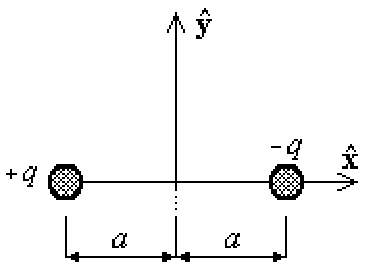
\includegraphics[width=\textwidth]{p1e05}
    \end{minipage}



\item Una molécula de agua tiene su átomo de oxígeno en el origen y los núcleos de hidrógeno en \(\vec{r}= (\pm\SI{0.077}{\nano\metre}; \SI{0.058}{\nano\metre} ) \).
% \item[Problema 14] Una molécula de agua tiene su átomo de oxígeno en el origen y los núcleos de hidrógeno en \(\vec{r}= (\pm\SI{0.077}{\nano\metre}; \SI{0.058}{\nano\metre} ) \).
Si los electrones del hidrógeno se transfieren completamente al átomo de oxígeno, ¿cuál sería el momento dipolar de la molécula?
Compare con el valor experimental (esta caracterización de los enlaces químicos del agua como totalmente iónicos sobrestima el momento dipolar).


\item Un anillo de radio R está cargado uniformemente con una carga total \(–q\).
% \item [Problema 15] Un anillo de radio R está cargado uniformemente con una carga total \(–q\).
En el centro del mismo se coloca una carga puntual \(q\).
\begin{enumerate}
  \item ¿Cuánto valen los momentos monopolar y dipolar?
¿Depende el momento dipolar del origen de coordenadas?
  \item Calcule el potencial y el campo eléctrico sobre el eje del anillo y estudie el comportamiento a distancias grandes.
\end{enumerate}



\end{enumerate}
% \end{description}
\end{document}
